\documentclass[a4paper, 10pt]{article}
\usepackage[siunitx]{circuitikz}
\usepackage[margin=1in]{geometry}
\usepackage{subfiles}

\usetikzlibrary{intersections}

\tikzset{blockdef-above/.style={%
	{Straight Barb[harpoon, right, length=-0.2cm]}-{Straight Barb[harpoon, left, length=-0.2cm]},
	black,
	}}

\tikzset{blockdef-below/.style={%
	{Straight Barb[harpoon, reversed, right, length=0.2cm]}-{Straight Barb[harpoon, reversed, left, length=0.2cm]},
	black,
	}}

\def\gateTransistor{$BC547$}
\def\baseResistor{\SI{220}{k\ohm}}
\def\outResistor{\SI{47}{k\ohm}}
\def\ledResistor{\SI{18}{k\ohm}}
\def\vccPotential{$V_{CC}=\SI{5}{V}$}

\begin{document}

\section{Logic Gates}

\subsection{AND Gate}

\begin{figure}[!ht]
	\centering
    \includegraphics{tikzpics/epictlvlandgate.pdf}
	\caption{\textbf{AND} Gate}
\end{figure}

\subsection{OR Gate}

\begin{figure}[!hb]
	\centering
    \includegraphics{tikzpics/epictlvlorgate.pdf}
	\caption{\textbf{OR} Gate}
\end{figure}

\subsection{XOR Gate}

\begin{figure}[!hp]
	\centering
    \includegraphics{tikzpics/epictlvlxorgate.pdf}
	\caption{\textbf{XOR} Gate}
\end{figure}

\clearpage

\section{Adders}

\subsection{Half Adder}

\begin{figure}[!ht]
	\centering
    \includegraphics{tikzpics/epicglvlhalfadder.pdf}
	\caption{Half Adder}
\end{figure}

\vspace{0.2\textheight}

\subsection{Full Adder}

\begin{figure}[!hb]
	\centering
    \includegraphics{tikzpics/epicglvlfulladder.pdf}
	\caption{Full Adder}
\end{figure}

\clearpage

\subsection{Full Adder from Raw \textbf{Transistors}}

\begin{figure}[!h]
	\centering
	\resizebox{\textwidth}{!}{
    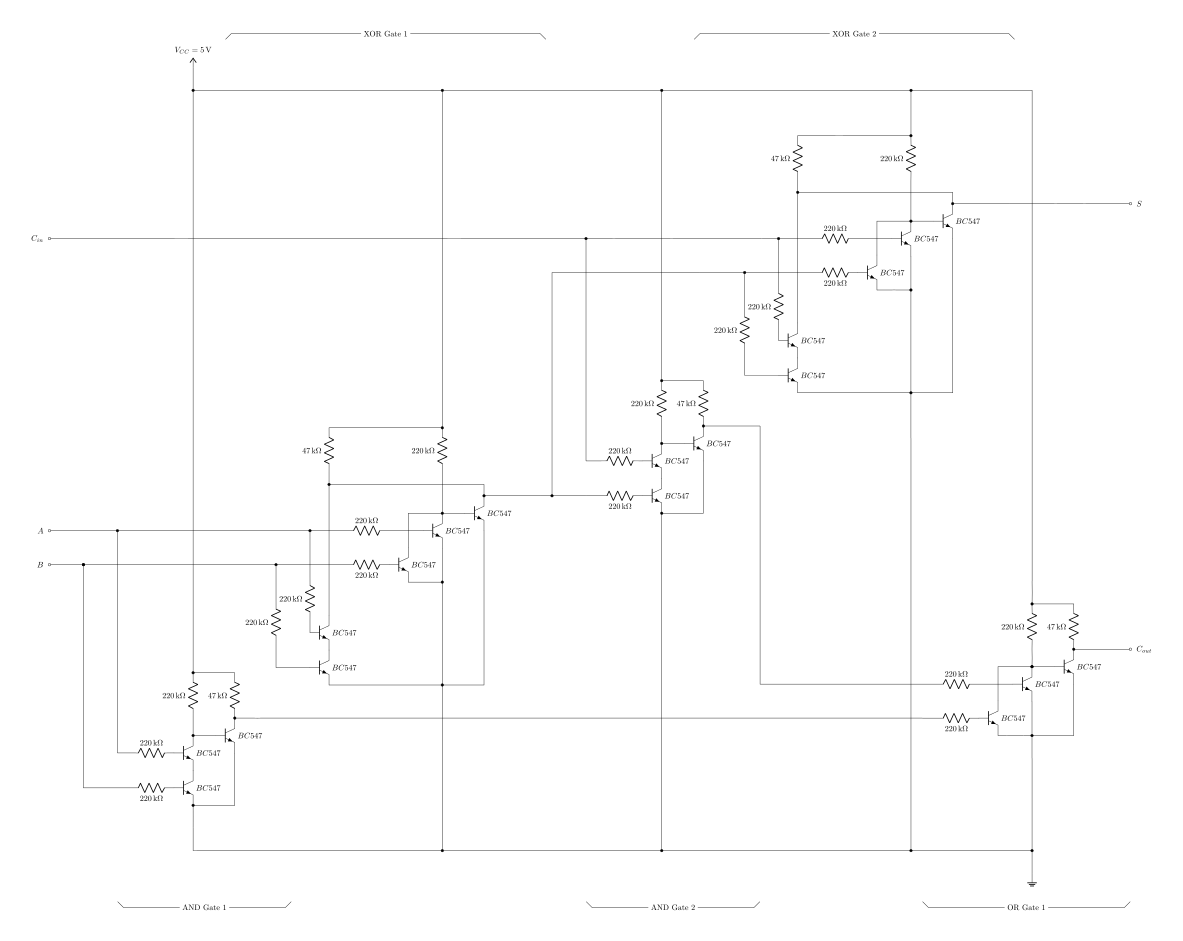
\includegraphics{tikzpics/epictlvlfulladder.pdf}
	}
	\caption{Full Adder from Raw \textbf{Transistors}}
\end{figure}

\clearpage

\section{Control Unit}

\subsection{Control Unit for 4 bit Ripple Adder}

\begin{figure}[!h]
    \centering
    \resizebox{!}{0.8\textheight}{
        \includegraphics{tikzpics/epicfourbitaddercu.pdf}
    }
    \caption{Control Unit for \textbf{4 bit Ripple Adder}}
\end{figure}


\clearpage

\subsection{Control Unit for Full Adder}

\begin{figure}[!h]
	\centering
	\resizebox{\textwidth}{!}{
        \includegraphics{tikzpics/epicfulladdercu.pdf}
	}
	\caption{Control Unit for \textbf{Full Adder}}
\end{figure}

\end{document}
